\chapter{Introduction}
According to the Reuters Institute, 36\% of French adults use social media as a source of news.\footnote{\url{http://media.digitalnewsreport.org/wp-content/uploads/2018/06/digital-news-report-2018.pdf?x89475}}  This share has declined since 2017, but this is mostly due to a decrease in the use of Facebook, while other networks are stable (like Twitter) or growing rapidly. This evolution of news consumption may reflect a growing interest for stories that are usually not covered by traditional news media, or that are covered in a different way. This raises the question of the type of news that is mostly shared on social networks: are the citizens differently informed when they use social network as a gateway to news? 

In response to the transformation of news consumption, one should expect a change in the production of news by traditional media outlets. \citet{mcgregor_twitter_2018} find that journalists using Twitter as part of their daily work consider tweets as newsworthy as headlines from the Associated Press. Does this change in the perception of journalists has an effect on the type of stories they choose to report? Does the success of a story on social media impacts the news production by traditional news media outlets?


The objective of this thesis is to investigate the role of Twitter in the evolution of both news consumption and news production in recent years. We aim at understanding what kind of news are  amplified by the sphere of social networks, and, conversely, to show in which cases events born on the social networks become a subject relayed by traditional media outlets. The challenge is to quantify and analyze precisely the relationships between the two spheres, in a context of very strong influence of each sphere on the other. 


Indeed, stories do not spread only in one direction, from news media to social networks or from social networks to news media. The recent Benalla case in France can be used as an illustration of the different rebounds that an event can have in both spheres: videos of Alexandre Benalla wearing a police helmet and hitting a protester where published on social media on May 1, 2018. However, he was only identified as an aide from President Macron's office on July 18, by the newspaper \textit{Le Monde}. After this first article, traditional media outlets started to investigate on the missions of Mr. Benalla. Both journalists and Twitter users published numerous pictures of Alexandre Benalla in official appearances of the President, including during the period when he was allegedly suspended. The newspaper ``Sud Ouest" used the term ``photo hunt" to qualify the attitude of social media users and photo reporters\footnote{\url{https://www.sudouest.fr/2018/07/23/affaire-benalla-quand-les-reseaux-sociaux-s-amusent-5256018-10458.php}}. On July 30, a Belgian organization called DisinfoLab evoked an artificial swelling of the number of messages on Twitter related to the Benalla case.\footnote{\url{https://twitter.com/DisinfoEU/status/1023903729668575242}} In the partial results published on that day, the ``overactivity" of some Twitter accounts and ``pro-Russian" accounts were mentioned. On August 8, DisinfoLab published the entire study,\footnote{\url{https://spark.adobe.com/page/Sa85zpU5Chi1a/}} showing no evidence that an organized Russian intervention has sought to amplify the Benalla case on Twitter. However, several media outlets had already relayed the (wrong) information that ``Russian bots"  had influenced the reaction of the public on Twitter.\footnote{\url{https://abonnes.lemonde.fr/les-decodeurs/article/2018/08/08/l-impossible-quete-des-bots-russes-de-l-affaire-benalla_5340540_4355770.html?}}


%%%%%%%%%%%%%%%%%%%%%%%%
\begin{figure}
\begin{center}
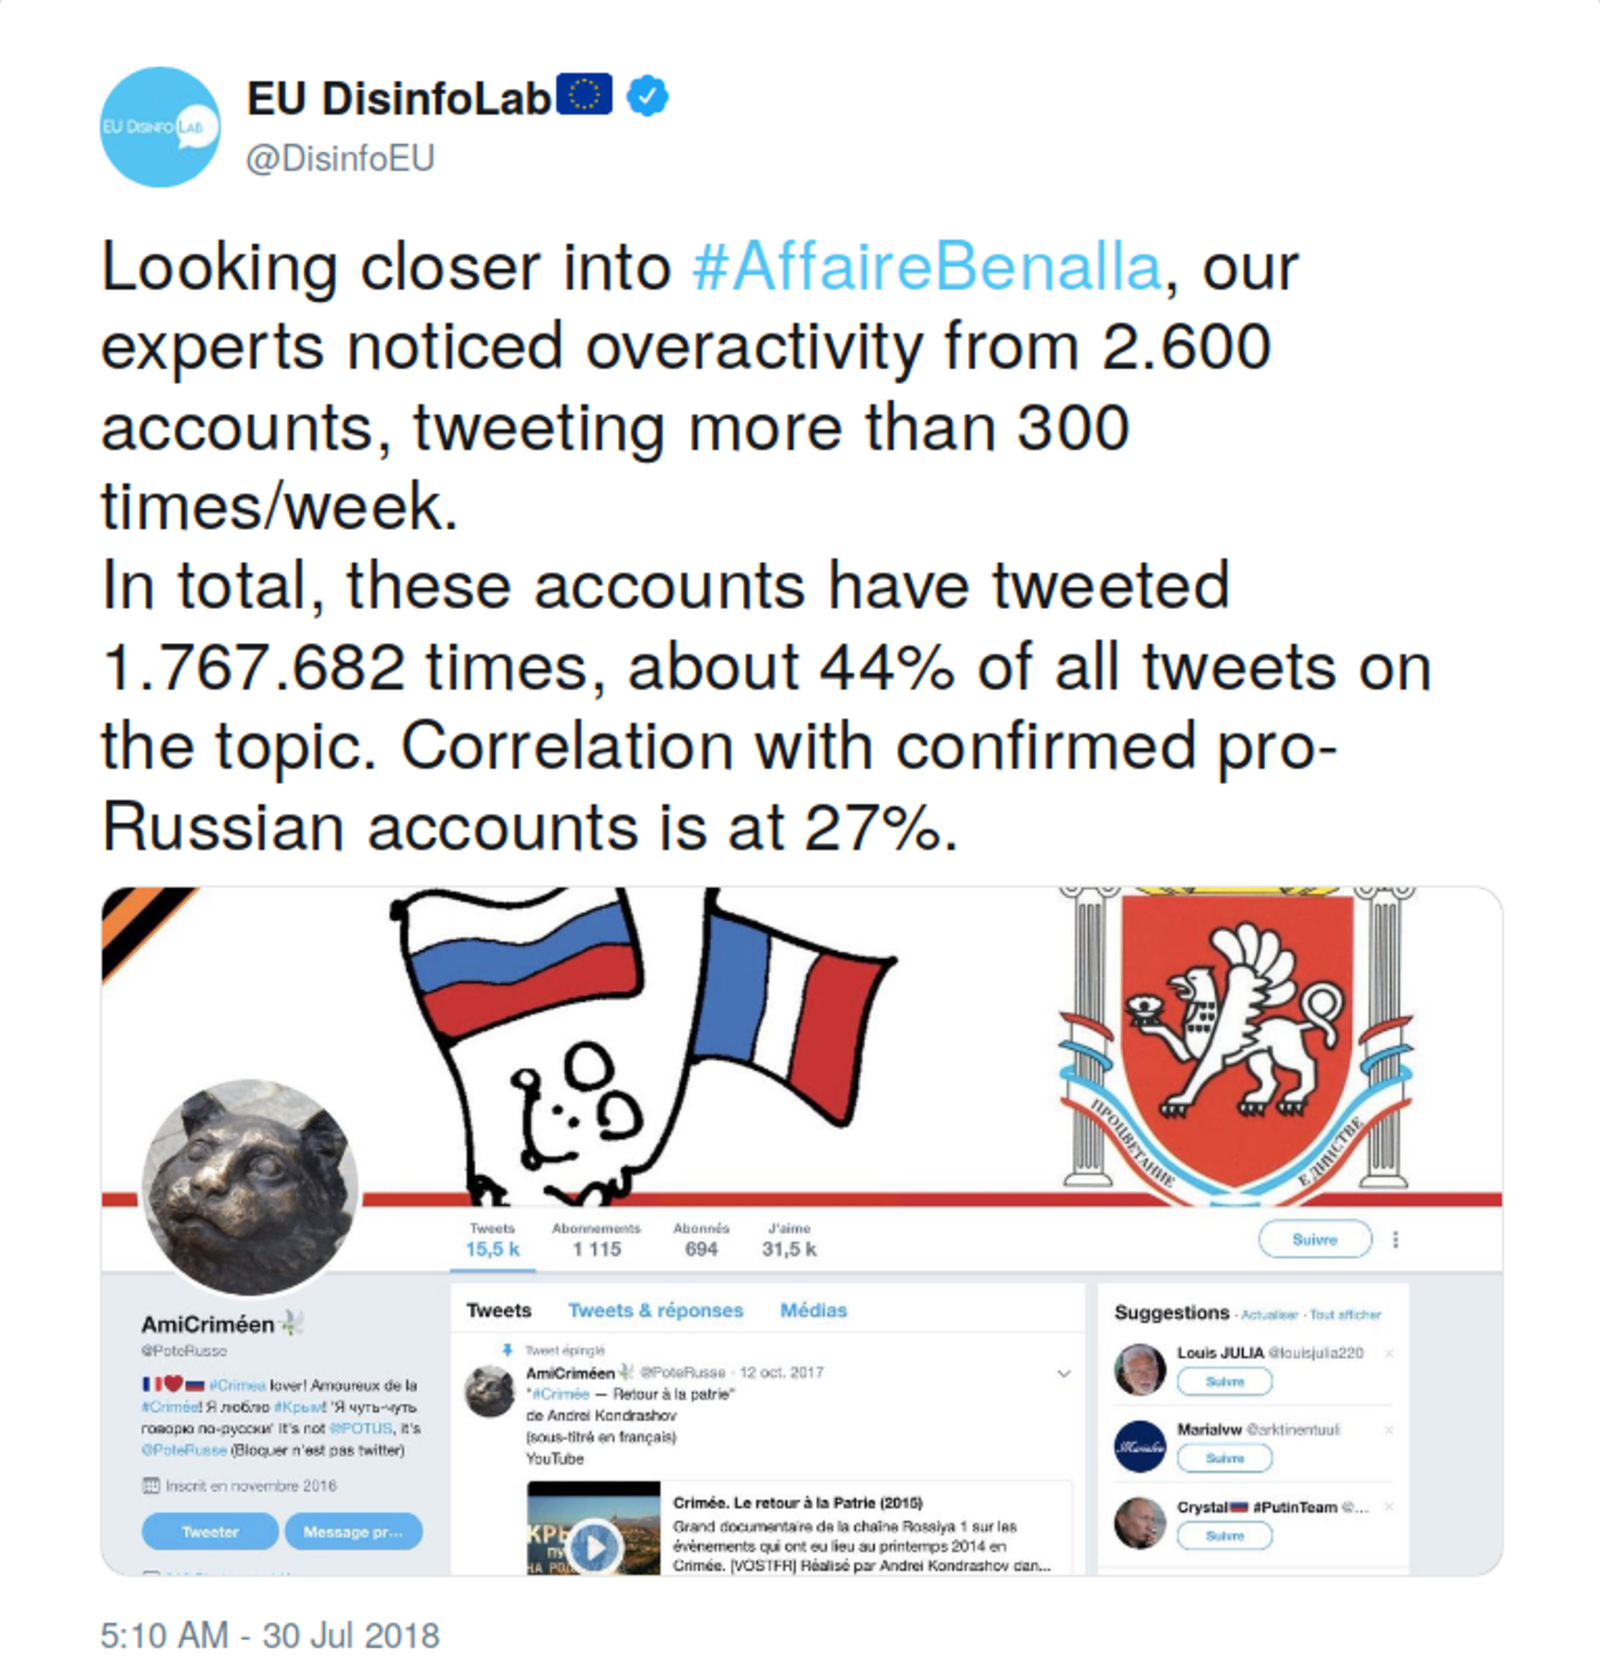
\includegraphics[scale=.35]{figures/Screenshot_DisinfoLab_AffaireBenalla.pdf}
\end{center}
{\scriptsize \textbf{Notes:} These preliminary results were nuanced in the full study published on August 8, 2018}
\caption{Tweet from DisinfoLab, an organization working on disinformation, about the ``overactivity" of some Twitter accounts during the Benalla scandal}
\label{Figure:DisinfoLab}
\end{figure}
%%%%%%%%%%%%%%%%%%%%%%%%

This is only one example of the plurality of ``interaction patterns" \citep{ning_uncovering_2015} between social networks and traditional media that can occur in the news agenda. Here, social networks are first used as a source by news outlets (most videos of Alexandre Benalla used by journalists where initially published on Twitter by witnesses of the May 1 demonstration). Then, they participate to the controversy raised by traditional media outlets and amplify it. Finally, the amplitude of the echo on Twitter is discussed by media outlets. Other types of interaction patterns exist, for example ``break on Twitter first" stories (like the hashtag \#MakeOurPlanetGreatAgain posted on June 2017 by Emmanuel Macron that was widely commented by traditional news media) or Twitter movements that criticize traditional media (for example, Twitter users reacted to the shocking images of victims of the Nice attack with the hashtag \#CSACoupezTout, which led the \textit{France Télévisions} group to apologize\footnote{\url{https://www.francetvinfo.fr/economie/medias/france-televisions/edition-speciale-sur-l-attentat-de-nice-france-televisions-presente-ses-excuses_1548057.html}}). We aim at developing measurement tools and analysis criteria to characterize and quantify these interaction patterns.


The originality of this project is its bi-disciplinary nature. On the one hand, it will consist of an analysis in media economics, in order to determine the factors that influence the relative impact of a story on Twitter and in traditional news media. This thesis will have to take into account several types of measures of the media impact, both absolutely (number of tweets, number of articles), but also related to the membership networks of the users emitting the information:  a story spreads more widely if it is issued within a majority group \citep{HalberstamKnight2016}, and information is more easily relayed if it emanates from the account of a journalist or a politician \citep{harder_making_2016}. On the other hand, it will require advanced computer science research to design novel approaches to Twitter event detection and clustering, using both Natural Language Processing and Image Processing.


\section{Choice of Twitter}
Why choose Twitter over another social network? Twitter is a micro-blogging website where users can post short messages called ``tweets". Tweets are limited to 280 characters, but can also contain pictures or videos. It is difficult to find reliable statistics on the number of tweets emitted every day worldwide. In 2014, Twitter announced the figure of 500 million tweets on average per day\footnote{\url{https://blog.twitter.com/official/en_us/a/2014/the-2014-yearontwitter.html}}, but there has been no other official statement since.   Several types of interactions are possible on this social network: users can ``follow" other users (that is to say, subscribe to their account in order to see all the tweets they publish), they can ``retweet" a tweet (re-publish it on their own account), ``reply" to it, ``quote" it (re-publish the tweet with a comment of their own) or ``like" it. Users can refer to other users in their tweets using ``mentions" (the user's name preceded by "@"), and they can tag specific words as important using ``hashtags" (words preceded by ``\#"). Tweets are publicly visible by default, which is why Twitter is used by many public personalities like politicians or journalists. This is one of the main differences between Twitter and Facebook, where posts can by default only be read by one's ``friends" (usually people that one know in real life).

	
	Twitter is not the most used social network in France. According to the Reuters Intitute, in 2018 it is even the 4th French social network (used by 16\% of respondents), behind Facebook (63\%), YouTube (51\%) and Facebook Messenger (31\%). Nevertheless, we chose this network for our analysis of the relationships between social networks and traditional news media for several reasons. 

	
	First of all, it is predominantly used for news access. The ``News Use Across Social Media Platforms 2018" study by the Pew Research Center\footnote{\url{http://www.journalism.org/2018/09/10/news-use-across-social-media-platforms-2018/}} finds that 71\% of American Twitter users get news on the platform, compared to 68\% for Facebook and 38\% for YouTube. There is no similar study on French social networks, but the structure of Twitter makes it a privileged tool for sharing news content, independently of the country. Indeed, if favors public statements rather than private messages to family and friends, and encourages the sharing of external content (reference to other pages through URLs) because of the brevity of tweets. \citet{kwak_twitter_2010} even argue that the structure of Twitter makes it similar to a news media.
	
	
	Secondly, Twitter has quickly become the preferred network of journalists, who use it both to easily contact sources and to build a connection with their audience \citep{swasy_little_2016}. In the sample of journalists studied by \citet{mcgregor_twitter_2018}, 93\% had a Twitter account. A report conducted at the request of the European Commission\footnote{\url{http://ec.europa.eu/commfrontoffice/publicopinion/archives/quali/journsm_en.pdf}} shows a similar trend in Europe: the interviewed journalists make the distinction between Twitter, mostly used for work, and Facebook, more used in private life.
	
	
	Finally, Twitter provides a larger access to its data than other social media platforms. Even if the volume of tweets that one can access through Twitter's APIs is limited, the company still provides a free access to a rather large volume of data. Conversely, despite the research effort recently launched by Facebook to protect elections,\footnote{\url{https://www.facebook.com/notes/mark-zuckerberg/preparing-for-elections/10156300047606634/}} it is still nearly
impossible for researchers outside Facebook to get access to information on users' activity on the platform.

\section{Choice of France}
Working on French tweets and news contents is difficult due to the still little amount of available corpora for Natural Language Processing and tweet analysis compared to English. However, we can rely on the corpus provided by the French Institute for Audiovisual (INA) that contains all content published by French news media online (newspapers, radio, televisions and online pureplayers) with their precise publication date \citep{cage2020production}. 
Besides, we have access to the universe of the AFP (Agence France Presse) news agency’s dispatches,
which gives us a proxy for the news stories that make it to traditional media outlets – with similarly the exact time of each dispatch. 


Besides, the main empirical challenge for researchers
using Twitter data comes from the fact that, because of the limits of the Twitter streaming
API, it is impossible for researchers to capture the universe of tweets that are posted on the
platform during a given period of time. Perhaps paradoxically, the advantage of France comes
here from the fact that there is less data than for example for the United States: according to our estimates, around 9.2 million tweets are published every day in French. Using the collection methods detailed in chapter \ref{Building Corpus} section \ref{Subsec: collection strategy}, we are able to capture a little bit more than 4.5 million tweets a day, which means that our dataset covers nearly half of all the tweets published in French.

\section{Characterization of events}
\color{orange}
What is a media event? One possible definition is: a fact that is important enough to be reported in the media. In contemporary societies, news media have therefore a role to play in the definition of events.  According to the historian Pierre Nora, the emergence of the mass media has transformed the nature of events: \textit{``Press, radio, images are not only means from which events would be relatively independent, they are the very condition of their existence."}\footnote{``Presse, radio, images, n'agissent pas seulement comme des moyens dont les événements seraient relativement indépendants, mais comme la condition même de leur existence."}\citep{nora_evenement_1972}. The sociologist Patrick Champagne \citep{champagne_evenement_2000} shares the same view (\textit{``The media build the events they report"}\footnote{``les médias construisent les événements dont ils rendent compte"}) but highlights the fact that creating an event is a collective process : one media outlet alone cannot make the news if it is not picked up by others. A media event has thus to be reported by several sources to be defined as such.


With the appearance of social media, a new dimension has emerged: traditional news media cannot ignore a topic that is really bursting on Facebook or Twitter. In practice, many news events start nowadays on social media, like the \#MeToo movement.  Social events and media events tend to be the same in many cases, that is what we call \textit{joint events}. However, any conversation or trend on social media cannot be considered as a \textit{media event}. We therefore propose a distinction between \textit{media events, social events} and \textit{joint events} In this part, we  provide definitions that formalize these intuitions.

\subsection{Definitions \label{Subsec: Definitions}}


\subsubsection{Literature review}
			There is no consensus on the formal definition of the problem of event detection on Twitter, mainly because of the diversity of use-cases and scenarios for which event detection may be useful. \citet{sankaranarayanan_twitterstand:_2009} aim at providing a user interface displaying breaking news from tweets in the same way as a news wire. \citet{aiello_sensing_2013} design their tool for ``an expert of some domain [who] has to monitor specific topics or events being discussed in social media". \citet{zhang_triovecevent:_2017} give several applications of their event detector, such as sending alarms in case of imminent disaster or helping local governments to prevent social unrest. These few examples highlight the fact that all authors working on the subject do not perceive \textit{``event detection"} in the same way: their tools do not detect the same \textbf{type of events} (local events, conversations about specific topics, breaking news...), they do not have the same \textbf{inputs} (tweets from a range of selected sources, geo-tagged tweets, tweets containing a given keyword...) and \textbf{outputs} (all detected events, the top $k$ events depending on some relevance criteria, a list of tweets linked to each event, a list of keywords...), and are not designed to handle the same \textbf{volume of tweets}. We propose here an overview of the existing definitions.
			
Even though it is not focused on tweets but rather on traditional news contents, many articles on Twitter event detection refer to the definition given in the Topic Detection and Tracking project \citep{allan_introduction_2002}: an event is ``something that happens at a specific time and place along with all necessary conditions and unavoidable consequences". 
For \citet{aggarwal_event_2012} and \citet{mcminn_building_2013}, the definition of event is similar but includes another dimension: an event has to be ``of interest to the news media" \citep{aggarwal_event_2012}.
\citet{becker_beyond_2011} consider that events are necessarily linked to a real world fact: they define an event as ``a real-world occurrence $e$ with (1) an associated time-period $T_e$ and (2) a time-ordered stream of Twitter messages $M_e$, of substantial volume, discussing the occurrence and published during time $T_e$."  
 For \citet{hasan_survey_2018}, the notion of ``real world" is also mentioned. An event is ``an occurrence of interest in the real world which instigates a discussion on the event-associated topic by various users of social media, either soon after the occurrence or, sometimes, in anticipation of it." 
 In these definitions, the events have to exist outside social medias: they have to be either mentioned by other traditional media outlets, or be linked to an ``occurrence", a ``fact" in the real world.
 
Other authors define a social media event depending on the actions they generate on the studied social media. \citet{panagiotou_detecting_2016} call ``action" any activity on a social media, such as posting new content, interacting with another profile (sending a friend request, for example) or interacting with existing contents (like, or retweet). In their definition, an event is ``something that causes a large number of actions in the OSN [Online Social Network]". This type of approaches often consider events as ``breaking news" that will generate a larger activity on social media than any other topic at a given moment. This is also the approach of \citet{guille_event_2015}, that focus on detecting ``bursty" patterns.

For our study, we need to detect on Twitter any set of tweets from several sources that discuss the same fact. These facts do not have to exist outside of the social media (in the so called ``real world"). Besides, defining an event depending on its ``burstiness" can lead to neglect smaller size events.

Let $f$ be a \textbf{triggering fact}, i.e. a fact that causes an
important \textbf{activity} in either the traditional media sphere or the social media sphere or the both. This fact can happen in real life or on the internet. \citet{panagiotou_detecting_2016} discuss the relevance of a distinction between \textit{real world events} and \textit{virtual events} such as ``memes, trends or popular discussions". These distinctions are unnecessary for our applications: for example, many politicians use social media to make public statements, that are not less ``real" than the ones made during interviews or press conferences. A triggering fact can thus be a tweet, a Youtube video, a speech, a sport performance, a trial, a Facebook post, etc.


In our work, we consider that a \textbf{source} $s$ can be a media outlet or a Twitter account. A \textbf{source} can publish one or several \textbf{content objects}.


A \textbf{content object} $o$ is a tuple $(x_o, s_o, d_o, f)$ with $x_o$ the object in itself (i.e. a  tweet, a news article,...), $s_o$ its source,
$d_o$ its publication date and $f$ the related triggering fact.

Two kinds of content object will be considered in this thesis :
\begin{itemize}
\item \textbf{Twitter object} $t =(x_t, s_t,d_t, f ) $ in which $x_t$ is the tweet
(text and /or visual contents) and $s_t$ is a Twitter account and $d_t$
the publication date of the tweet.
\item \textbf{Media object}  $m=(x_m,s_m,d_m,f)$ in which $x_m$ is the media content (press article, video, television or radio report...), $s_m$ is a media outlet, and $d_m$ the publication date of the object.
\end{itemize}
  
Using these different concept, we can now defined an \textbf{event} as a set of content objects from several sources that are related to the same fact $f$. 


More precisely, a \textbf{Twitter event} $E_T$ is a set of Twitter objects
$\{t_1,...,t_n\}$  discussing the same fact $f$ and generated by a least $k$ different sources (i.e. Twitter accounts) in a restricted time interval $[d_{start},d_{end}]$. For the sake of clarity, we introduce the set 
$X_T = \{x_t^1, ..., x_t^n\}$, 
$S_T = \{s_t^1, ... ,s_t^n\}$ and 
$D_T = [d_{t,start},d_{t,end}]$ that are respectively the
set of tweets, the set of sources and the time interval of $E_T$. $E_T$ is a Twitter event if $|S_T|  \geq k$ and if  $D_T 
\subseteq [d_{start},d_{end}]$.


Similarly, a \textbf{Media event} $E_M$ is a set of media objects
$\{m_1,...,m_n\}$  discussing the same fact $f$ and generated by a least $l$ different sources (i.e. media outlets) in a restricted time interval $[d_{start},d_{end}]$. We introduce the set 
$X_M = \{x_m^1, ..., x_m^n\}$, 
$S_M = \{s_m^1, ... ,s_m^n\}$ and 
$D_M = [d_{m,start},d_{m,end}]$ that are respectively the
set of tweets, the set of sources and the time interval of $E_M$. $E_M$ is a media event if $|S_M|  \geq l$ and if  $D_M 
\subseteq [d_{start},d_{end}]$.

\section{Detailed Outline}